\documentclass{article}
% For math environments
\usepackage{amsmath, amsfonts}
% For links
\usepackage[hidelinks]{hyperref}
% So space it put between paragraphs
\usepackage{parskip}
% For figures
\usepackage{tikz}
% Set the margins to not be ridiculous
\usepackage[margin=0.75in]{geometry}
% For multiple columns
\usepackage{multicol}
% For controlling enum/itemize spacing and indentation
\usepackage{enumitem}

% For tikz plots
\usepackage{pgfplots}
% This isn't needed but avoids a compiler warning
\pgfplotsset{compat=1.16}

% Allow multi-line equations to be broken across pages
\allowdisplaybreaks

% Use @ as a letter
\makeatletter

% Scale down all tikz coordinates while maintaining font size
\tikzset{every picture/.style={scale=0.45, every picture/.style={}}}


% Macros
% Monospace code
\def\code#1{\texttt{#1}}

% Greek letters
\def\a{\alpha}
\def\b{\beta}
\def\g{\gamma}
\def\d{\delta}
\def\D{\Delta}

% Some common sets
\def\es{\varnothing}
\def\ints{{\mathbb{Z}}}

% Commands that make life easier
\newcommand\gath[1]{\begin{gather} #1 \end{gather}}
\newcommand\gaths[1]{\begin{gather*} #1 \end{gather*}}
\newcommand\ali[1]{\begin{align} #1 \end{align}}
\newcommand\parens[1]{\left( #1 \right)}
\newcommand\squares[1]{\left[ #1 \right]}
\newcommand\braces[1]{\left\{ #1 \right\}}
\newcommand\angles[1]{\left\langle #1 \right\rangle}
\newcommand\deriv[2]{\frac{d #1}{d #2}}
\newcommand\abs[1]{\left| #1 \right|}
\newcommand\floor[1]{\left\lfloor #1 \right\rfloor}
\newcommand\ceil[1]{\left\lceil #1 \right\rceil}
\DeclareMathOperator{\lcm}{lcm}
\def\non{\nonumber \\}
\newcommand\unit[1]{~\mathrm{#1}}
\newcommand\combos[2]{{}_{#1}C_{#2}}

% Set stuff
\def\ss{\subseteq}

% Multiline equation space
\def\mlesp{\hspace{1.2cm}}

% For grid diagrams
\newcommand\gridbox[3]{\draw (#1,#2) rectangle (#1+1,#2+1) node[pos=.5] {#3};}
\newcommand\gridboxh[3]{\draw[fill=red!20] (#1,#2) rectangle (#1+1,#2+1) node[pos=.5] {#3};}
\newcommand\gridboxb[3]{\draw[fill=black] (#1,#2) rectangle (#1+1,#2+1) node[pos=.5] {#3};}
\newcommand\gridsym[3]{\node at (#1+0.5,#2+0.5) {$#3$};}
\newcommand\gridblank[2]{\filldraw[draw=gray, color=gray] (#1,#2) rectangle (#1+1,#2+1);}
\newcommand\gridcirc[2]{\draw (#1 + 0.5,#2 + 0.5) circle (0.25);}
\newcommand\cwlab[3]{
  \def\dd{0.15}
  \draw (#1 + \dd - 0.03, #2 + 1 - \dd) node {\scriptsize #3};
}

\def\bbw{3.5}
\def\bbh{2}
\newcommand\bigbox[3]{\draw (#1*\bbw,#2*\bbh) rectangle (#1*\bbw+\bbw,#2*\bbh+\bbh) node[pos=.5] {#3};}
\newcommand\bbtextr[3]{\node[right] at (#1*\bbw,#2*\bbh+0.5*\bbh) {#3};}
\newcommand\bbtextb[3]{\node[align=center] at (#1*\bbw+0.5*\bbw,#2*\bbh+0.5*\bbh) {#3};}

% Box puzzle stock answer
\newcommand\boxans[1]{
  Logic was used to deduce the solution:

  #1

  This was verified using Python as well as shown to be unique with a brute force approach.
}

% Standard crossnumber grid
\newcommand\crossnumstd[9]{
  \begin{center}
    \begin{tikzpicture}[scale=2]
      \gridbox{0}{2}{#1}
      \gridbox{1}{2}{#2}
      \gridbox{2}{2}{#3}
      \gridbox{0}{1}{#4}
      \gridbox{1}{1}{#5}
      \gridbox{2}{1}{#6}
      \gridbox{0}{0}{#7}
      \gridbox{1}{0}{#8}
      \gridbox{2}{0}{#9}

      % Labels
      \cwlab{0}{2}{1}
      \cwlab{1}{2}{2}
      \cwlab{2}{2}{3}
      \cwlab{0}{1}{4}
      \cwlab{0}{0}{5}
    \end{tikzpicture}
  \end{center}
}

% Multiple numbers
\newcommand\mn[1]{$#1$'s}

% Commands for problems
\newcommand\problem[4]{
\section*{#1}

\textbf{Question:} #3

\textbf{Answer:} #2

\textbf{Explanation:} #4
}
\newcommand\aproblem[4]{\problem{Dec #1}{#2}{#3}{#4}}
\newcommand\cproblem[4]{\problem{Problem #1}{#2}{#3}{#4}}

\newcommand\xref@advent[2]{#1 Advent, Dec~#2 problem}
\newcommand\xref@card[2]{#1 Christmas Card, Problem #2}

% For answered verified with Python
\newcommand{\verified}{This was verified with a brute-force Python program.}

\def\advent@xxi@i{
  The geometric mean of a set of $n$ numbers can be computed by multiplying together all the numbers then computing the $n$th root of the result.

  The factors of $4$ are $1$, $2$ and $4$. The geometric mean of these is 2.

  The factors of $6$ are $1$, $2$, $3$, and $6$. The geometric mean of these is $\sqrt{6}$.

  The geometric mean of all the factors of today's number is $22$.
}

\def\advent@xxi@ii{
  The number $7n$ has $37$ factors (including $1$ and the number itself).
  How many factors does $8n$ have?
}

\def\advent@xxi@iii{
  If you write out the numbers from $1$ to $1000$ (inclusive), how many times will you write the digit $0$?
}

\def\advent@xxi@iv{
  Put the digits $1$ to $9$ (using each digit exactly once) in the boxes so that the sums are correct.
  The sums should be read left to right and top to bottom ignoring the usual order of operations.
  For example, $4 + 3 \times 2$ is $14$, not $10$.
  Today's number is the product of the numbers in the red boxes.

  \grid@advent@xxi@iv{}{}{}{}{}{}{}{}{}
}

\def\advent@xxi@v{
  How many different isosceles triangles are there whose perimeter is $50$ units, and whose area is an integer number of units squared?

  (Two triangles that are rotations, reflections and translations of each other are counted as the same triangle. Triangles with an area of 0 should not be counted.)
}

\def\advent@xxi@vi{
  When $12345$ is divided by today's number, the remainder is $205$.
  When $6789$ is divided by today's number, the remainder is $112$.
}

\newcommand\dec@ai{0.30901699437494745}
\newcommand\dec@aii{0.8090169943749475}
\newcommand\dec@bi{0.5877852522924731}
\newcommand\dec@bii{0.9510565162951535}
\newcommand\decagon[5]{
  \def\ai{\dec@ai*#3+#1}
  \def\aii{\dec@aii*#3+#1}
  \def\bi{\dec@bi*#3+#2}
  \def\bii{\dec@bii*#3+#2}
  \draw (#3+#1, #2) -- (\aii, \bi) -- (\ai, \bii) -- (-\ai, \bii) -- (-\aii, \bi) -- (-#3+#1, #2) -- (-\aii, -\bi) -- (-\ai, -\bii) -- (\ai, -\bii) -- (\aii, -\bi) -- cycle;
  \fill[fill=red] (-\ai, -\bii) -- (#4*#3+#1, #5*#3+#2) -- (\ai, -\bii) -- cycle;
}
\def\advent@xxi@vii{
  The picture below shows eight regular decagons.
  In each decagon, a red triangle has been drawn with vertices at three of the vertices of the decagon.

  \begin{center}
    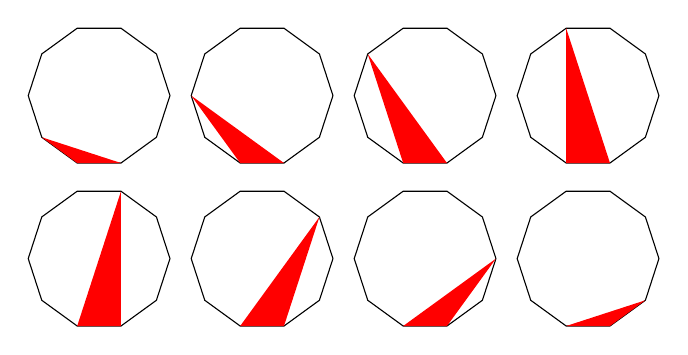
\begin{tikzpicture}
      \def\dr{2}
      \def\spc{2.3*\dr}

      \decagon{0*\spc}{\spc}{\dr}{-\dec@aii}{-\dec@bi}
      \decagon{1*\spc}{\spc}{\dr}{-1}{0}
      \decagon{2*\spc}{\spc}{\dr}{-\dec@aii}{\dec@bi}
      \decagon{3*\spc}{\spc}{\dr}{-\dec@ai}{\dec@bii}

      \decagon{0*\spc}{0}{\dr}{\dec@ai}{\dec@bii}
      \decagon{1*\spc}{0}{\dr}{\dec@aii}{\dec@bi}
      \decagon{2*\spc}{0}{\dr}{1}{0}
      \decagon{3*\spc}{0}{\dr}{\dec@aii}{-\dec@bi}
    \end{tikzpicture}
  \end{center}

  The area of each decagon is $240$.
  What is the total area of all the red triangles?
}

\def\advent@xxi@viii{
  The sum of three integers is $51$.
  The product of the same three integers is $836$. What is the product of largest integer and the second-largest integer?
}

\def\advent@xxi@ix{
  Eve writes down a sequence of consecutive positive integers (she writes more than one number).
  The sum of the numbers Eve has written down is $844$.
  Today's number is the smallest integer that Eve has written down.
}

\def\advent@xxi@x{
  Put the digits $1$ to $9$ (using each digit exactly once) in the boxes so that the sums are correct.
  Today's number is the largest number you can make using the digits in the red boxes.

  \grid@advent@xxi@x{}{}{}{}{}{}{}{}{}
}

\def\advent@xxi@xi{
  The integers are written in a triangle as shown below:
  \begin{center}
    \begin{tabular}{ccccccc}
         &    &    & 1    &    &    &    \\
         &    & 2  & 3    & 4  &    &    \\
         & 5  & 6  & 7    & 8  & 9  &    \\
      10 & 11 & 12 & 13   & 14 & 15 & 16 \\
         &    &    & etc. &    &    &
    \end{tabular}
  \end{center}
  Today's number appears directly above the number $750$ in the triangle of integers.
}

\def\advent@xxi@abgrid{
  \begin{center}
    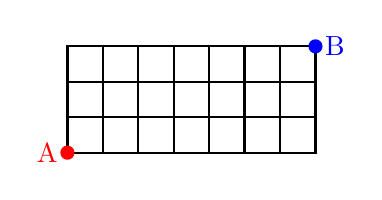
\begin{tikzpicture}
      \def\gs{1}
      % Grid
      \foreach \i in {0,...,6}{
          \foreach \j in {0,...,2}{
              \draw[thick] (\i * \gs, \j * \gs) rectangle (\i * \gs + \gs, \j * \gs + \gs);
            }
        }
      % Points
      \fill[color=red] (0, 0) circle (0.2) node[color=red,left] {A};
      \fill[color=blue] (7*\gs, 3*\gs) circle (0.2) node[color=blue,right] {B};
    \end{tikzpicture}
  \end{center}
}
\def\advent@xxi@xii{
  You start at the point marked A in the picture below. You want to get to the point marked B.
  You may travel \textbf{to the right} or \textbf{upwards} along the black lines.

  \advent@xxi@abgrid

  Today's number is the total number of possible routes to get from A to B.
}

\def\advent@xxi@xiii{
  The diagram below shows three circles and two triangles.
  The three circles all meet at one point.
  The vertices of the smaller red triangle are at the centers of the circles.
  The lines connecting the vertices of the larger blue triangle to the point where all three circles meet are diameters of the three circles.

  \begin{center}
    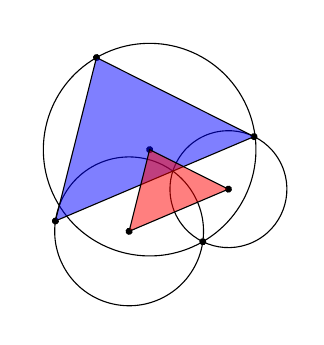
\begin{tikzpicture}[rotate=30,transform shape]
      \def\bcr{3}
      \def\scr{0.55*\bcr}
      \def\sca{34}
      \def\mcr{0.7*\bcr}
      \def\mca{142}
      \def\pr{0.1}

      % Circles
      \draw (0, \bcr) circle (\bcr);
      \draw (\sca: \scr) circle (\scr);
      \draw (\mca: \mcr) circle (\mcr);

      % Points
      \fill (0, 0) circle (\pr);
      \fill (0, \bcr) circle (\pr);
      \fill (0, 2*\bcr) circle (\pr);
      \fill (\sca: \scr) circle (\pr);
      \fill (\sca: 2*\scr) circle (\pr);
      \fill (\mca: \mcr) circle (\pr);
      \fill (\mca: 2*\mcr) circle (\pr);

      % Triangles
      \draw[fill=blue,fill opacity=0.5] (\mca: 2*\mcr) -- (0, 2*\bcr) -- (\sca: 2*\scr) -- cycle;
      \draw[fill=red,fill opacity=0.5] (\mca: \mcr) -- (0, \bcr) -- (\sca: \scr) -- cycle;
    \end{tikzpicture}
  \end{center}

  The area of the smaller red triangle is $226$.
  What is the area of the larger blue triangle?
}

\def\advent@xxi@xiv{
  You start at the point marked A in the picture below.
  You want to get to the point marked B.
  You may travel \textbf{to the right}, \textbf{upwards}, or \textbf{to the left} along the black lines, but you cannot pass along the same line segment more than once.

  \advent@xxi@abgrid

  Today's number is the total number of possible routes to get from A to B.
}

\newcommand\pyramid@advent@xxi@xvi[6]{
  \begin{center}
    \begin{tabular}{cccccc}
      (row 1) &    &    & #1   &    &    \\
      (row 2) &    & #2 &      & #3 &    \\
      (row 3) & #4 &    & #5   &    & #6 \\
              &    &    & etc. &    &
    \end{tabular}
  \end{center}
}
\def\advent@xxi@xv{
  The odd numbers are written in a pyramid.

  \pyramid@advent@xxi@xvi{1}{3}{5}{7}{9}{11}

  What is the mean of the numbers in the 19th row?
}

\newcommand\grid@advent@xxi@xvi[9]{
  \begin{center}
    \begin{tikzpicture}[scale=2]
      \gridbox{0}{2}{#1}
      \gridbox{1}{2}{#2}
      \gridbox{2}{2}{#3}
      \gridbox{0}{1}{#4}
      \gridbox{1}{1}{#5}
      \gridbox{2}{1}{#6}
      \gridbox{0}{0}{#7}
      \gridbox{1}{0}{#8}
      \gridbox{2}{0}{#9}

      % Labels
      \cwlab{0}{2}{1}
      \cwlab{1}{2}{2}
      \cwlab{2}{2}{3}
      \cwlab{0}{1}{4}
      \cwlab{0}{0}{5}
    \end{tikzpicture}
  \end{center}
}
\def\advent@xxi@xvi{
  Each clue in this crossnumber is formed of two parts connected by a logical connective: AND means that both parts are true; NAND means that at most one part is true; OR means that at least one part is true; NOR means that neither part is true; XOR means that exactly one part is true; XNOR means that either both parts are false or both parts are true.
  No number starts with $0$.

  \begin{multicols}{2}
    \grid@advent@xxi@xvi{}{}{}{}{}{}{}{}{}

    \columnbreak

    \begin{enumerate}
      \item \textbf{1A} is a palindrome XNOR \textbf{1D} is a palindrome.
      \item \textbf{1A} is greater than $350$ NOR \textbf{1D} is less than $150$.
      \item \textbf{3D} is odd NAND \textbf{4A} and \textbf{2D} are equal.
      \item \textbf{3D} is prime XOR \textbf{5A} is odd.
      \item \textbf{4A} is a cube AND \textbf{2D} is a cube.
      \item The sum of the digits of \textbf{3D} is $2$ OR the sum of the digits of \textbf{5A} is $5$.
      \item Today's number is \textbf{1D}.
    \end{enumerate}
  \end{multicols}
}

\def\advent@xxi@xvii{
  The digital product of a number is computed by multiplying together all of its digits. For example, the digital product of $6273$ is $252$.

  Today's number is the smallest number whose digital product is $252$.
}

\def\advent@xxi@xviii{
  Put the digits $1$ to $9$ (using each digit exactly once) in the boxes so that the sums are correct.
  The sums should be read left to right and top to bottom ignoring the usual order of operations.
  For example, $4 + 3 \times 2$ is $14$, not $10$.
  Today's number is the product of the numbers in the red boxes.

  \grid@advent@xxi@xviii{}{}{}{}{}{}{}{}{}
}

\def\advent@xxi@xix{
  The equation $352x^3 - 528x^2 + 90 = 0$ has three distinct real-valued solutions.

  Today's number is the number of integers $a$ such that the equation $352x^3 - 528x^2 + a = 0$ has three distinct real-valued solutions.
}

\def\advent@xxi@xx{
  What is the area of the largest area triangle that has one side of length $32$ and one side of length $19$?
}

\newcommand\grid@advent@xxi@xxi[9]{
  \begin{center}
    \begin{tikzpicture}
      \bigbox{0}{3}{#1}
      \bigbox{1}{3}{#2}
      \bigbox{2}{3}{#3}
      \bbtextr{3}{3}{\textbf{today's number}}

      \bigbox{0}{2}{#4}
      \bigbox{1}{2}{#5}
      \bigbox{2}{2}{#6}
      \bbtextr{3}{2}{prime}

      \bigbox{0}{1}{#7}
      \bigbox{1}{1}{#8}
      \bigbox{2}{1}{#9}
      \bbtextr{3}{1}{square}

      \bbtextb{0}{0}{cube}
      \bbtextb{1}{0}{odd}
      \bbtextb{2}{0}{multiple\\of $11$}
    \end{tikzpicture}
  \end{center}
}
\def\advent@xxi@xxi{
  Arrange the digits $1$–$9$ (using each digit exactly once) so that the three digit number in: the middle row is a prime number; the bottom row is a square number; the left column is a cube number; the middle column is an odd number; the right column is a multiple of $11$.
  The $3$-digit number in the first row is today's number.

  \grid@advent@xxi@xxi{}{}{}{}{}{}{}{}{}
}

\def\advent@xxi@xxii{
  There are $12$ ways of placing $2$ tokens on a $2 \times 4$ grid so that no two tokens are next to each other horizontally, vertically or diagonally:

  \begin{center}
    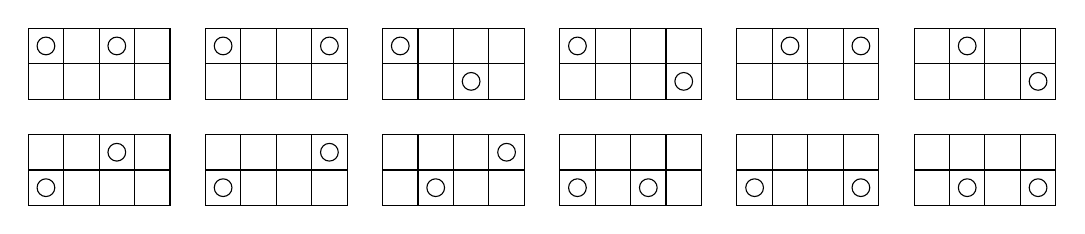
\begin{tikzpicture}
      % Draw all the grids
      \foreach \gi in {0,1}{
          \foreach \gj in {0,...,5}{
              \foreach \i in {0,1}{
                  \foreach \j in {0,...,3}{
                      \gridbox{5*\gj + \j}{3*\gi + \i}{}
                    }
                }
            }
        }

      % Place token circles
      \gridcirc{0}{4}
      \gridcirc{2}{4}
      \gridcirc{5}{4}
      \gridcirc{8}{4}
      \gridcirc{10}{4}
      \gridcirc{12}{3}
      \gridcirc{15}{4}
      \gridcirc{18}{3}
      \gridcirc{21}{4}
      \gridcirc{23}{4}
      \gridcirc{26}{4}
      \gridcirc{28}{3}
      \gridcirc{0}{0}
      \gridcirc{2}{1}
      \gridcirc{5}{0}
      \gridcirc{8}{1}
      \gridcirc{11}{0}
      \gridcirc{13}{1}
      \gridcirc{15}{0}
      \gridcirc{17}{0}
      \gridcirc{20}{0}
      \gridcirc{23}{0}
      \gridcirc{26}{0}
      \gridcirc{28}{0}
    \end{tikzpicture}
  \end{center}

  Today's number is the number of ways of placing $2$ tokens on a $2 \times 21$ grid so that no two tokens are next to each other horizontally, vertically or diagonally.
}

\def\advent@xxi@xxiii{
  I draw the parabola $y = x^2$ and mark points on the parabola at $x = 17$ and $x = -6$.
  I then draw a straight line connecting these two points.

  At which value of $y$ does this line intercept the $y$-axis?
}

\def\advent@xxi@xxiv{
  The digital product of a number is computed by multiplying together all of its digits.
  For example, the digital product of $1522$ is $20$.

  How many $12$-digit numbers are there whose digital product is $20$?
}

\def\card@xxi@i{
  What is the sum of all the odd integers between $0$ and $30$?
}

\def\card@xxi@ii{
  What is the sum of all the odd integers between $0$ and $5668$?
}

\def\card@xxi@iii{
  What is the smallest integer with a digital sum of $28$ and a digital product of $10000$?
}

\def\card@xxi@iv{
  What is the smallest integer with a digital sum of $41$ and a digital product of $432000$?
}

\def\card@xxi@v{
  What is the area of the largest area dodecagon that will fit inside a circle with area $111185 \pi$?
}

\def\card@xxi@vi{
  What is the area of the largest area heptagon that will fit inside a semicircle with area $115185 \pi$?
}

\def\card@xxi@vii{
  How many terms are there in the (simplified) expansion of $(x + y + z)^2$?
}

\def\card@xxi@viii{
  How many terms are there in the (simplified) expansion of $(x + y + z)^{41172}$?
}

\def\card@xxi@ix{
  What is the largest integer that cannot be written as $4a + 5b$ for non-negative integers $a$ and $b$?
}

\def\card@xxi@x{
  What is the largest integer that cannot be written as $83409a + 66608b$ for non-negative integers $a$ and $b$?
}

\def\card@xxi@xi{
  How many positive integers are there below $100$ whose digits are all non-zero and different?
}

\def\card@xxi@xii{
  How many positive integers are there whose digits are all non-zero and different?
}

\def\card@xxi@xiii{
  What is the only integer for which taking the geometric mean of all its factors (including $1$ and the number itself) gives $2$?
}

\def\card@xxi@xiv{
  What is the only integer for which taking the geometric mean of all its factors (including $1$ and the number itself) gives $25$?
}


\begin{document}

\title{MS Scroggs 2022 Christmas Card Solutions}
\author{Dan Whitman}
\date{}

\maketitle

Link to the online card: \href{https://www.mscroggs.co.uk/blog/98}{https://www.mscroggs.co.uk/blog/98}

\cproblem{1}{5}{\card@xxii@i}{
  Just working through the primes starting at $1$, the answer is clearly $5$, which is two more than $3$ and two less than $7$, both of which are also prime.
}

\newcommand\sumo[1]{s_\mathrm{o}\parens{#1}}
\cproblem{2}{49}{\card@xxii@ii}{
  While this would be really simple to just manually calculate, it is more fun (though perhaps more work) to derive an easier formula.
  Clearly the sum of the first $n$ odd numbers is going to be
  \gath{
    \sumo{n} = \sum_{k=1}^n (2k - 1) = 2 \sum_{k=1}^n k - \sum_{k=1}^n 1 = \frac{2n(n+1)}{2} - n = n^2 \,.
  }
  Thus our answer is $\sumo{7} = 7^2 = 49$.
}

\cproblem{3}{33}{\card@xxii@iii}{
  From the equation derived in the previous problem, clearly the answer is $\sqrt{1089} = 33$.
}

\cproblem{4}{1}{\card@xxii@iv}{
  Since $7$ is prime, the quotient group $\ints/7\ints$ is cyclic, and indeed $4$ is a generator for it.
  From this it follows that \emph{any} integer can be obtained by adding only integer multiples of $4$ and $7$.
  As an example, clearly $2 \cdot 4 - 1 \cdot 7 = 1$, which is of course the smallest positive integer period.
}

\cproblem{5}{80}{\card@xxii@v}{
  This is similar to the previous problem, but not so straightforward because our two integers are not coprime.
  In particular, $\gcd(240, 400) = 80$ so that only integer multiples of $80$ are obtainable by adding integer multiples of $240$ and $400$.
  Hence, our answer is of course $80$, noting that $2 \cdot 240 - 1 \cdot 400 = 80$ as an example of how to attain this.
}

\cproblem{6}{20}{\card@xxii@vi}{
  Here we can leverage the solution of the 2022, Dec~6 problem.
  There, it was reasoned that, for a digital sum of $1 \leq s \leq 9$, the number of $m$-digit numbers with this digital sum and for which there are no nonzero digits is the recursive function
  \gath{
    N_m(s) = \begin{cases}
      1                             & m = 1         \\
      \sum_{j=m-1}^{s-1} N_{m-1}(j) & 1 < m \leq 9.
    \end{cases} \label{eqn:06:rec}
  }
  It was also derived that, in particular,
  \gath{
    N_3(s) = \frac{(s-1)(s-2)}{2}.
  }
  Hence, for $4$-digit numbers we have
  \ali{
    N_4(s) &= \sum_{j=3}^{s-1} N_3(j) = \sum_{j=3}^{s-1} \frac{(j-1)(j-2)}{2} = \frac{1}{2} \sum_{j=3}^{s-1} \parens{j^2 - 3j + 2} = \frac{1}{2} \parens{\sum_{j=3}^{s-1} j^2 - 3 \sum_{j=3}^{s-1} j + 2 \sum_{j=3}^{s-1} 1} \non
    &= \frac{1}{2}\squares{\frac{s(s-1)(2s-1)}{6} - (2^2 + 1^2) - \frac{3s(s-1)}{2} + 3(2 + 1) + 2(s-3)} \non
    &= \frac{1}{2}\squares{\frac{2s^3 - 12s^2 + 22s - 12}{6}} = \frac{s^3 - 6s^2 + 11s - 6}{6}.
  }
  So our answer is then $N_4(7) = 20$, which was also verified with a brute force search Python program.
}

\cproblem{7}{64}{\card@xxii@vii}{
  This is just like the previous problem except that we are looking at all positive integers instead of just the $4$-digit integers.
  Again, we can use the results of the 2022, Dec~6 problem, according to which this number for the general digital sum $s$ is
  \gath{
    N_s = \sum_{m=1}^s N_m(s). \label{eqn:07:Ns}
  }
  Just like the Dec~6 problem, we shall not undergo the tedium of computing $N_5(s)$, $N_6(s)$, or $N_7(s)$, but instead implement \eqref{eqn:07:Ns} along with the recursive function \eqref{eqn:06:rec} in Python to arrive at our answer $N_7 = 64$.
  As before, this result was also verified with a brute force search in the Python program.
}

\cproblem{8}{2836}{\card@xxii@viii}{
  Suppose that the original $4$-digit number has digits $d_3 d_2 d_1 d_0$, where of course $0 \leq d_i \leq 9$ for all $0 \leq i \leq 3$.
  Now, it \emph{has} to be that the least significant digit is the one that was removed since otherwise the sum would end in $d_0 + d_0 = 2d_0$ so that it would have to end in an even digit.
  Since the sum
  ends in a $9$ though, it must be that the $3$-digit number is $d_3 d_2 d_1$, and our sum is
  \begin{center}
    \begin{tabular}{ccccc}
          & $d_3$ & $d_2$ & $d_1$ & $d_0$ \\
      $+$ &       & $d_3$ & $d_2$ & $d_1$ \\
      \hline
          & 3     & 1     & 1     & 9
    \end{tabular}
  \end{center}
  Clearly either $d_3 = 3$ and nothing is carried from the $d_2 + d_3$ digit, or else $d_3 = 2$ and a $1$ \emph{is} carried.
  It must be the latter case since, in the former case, clearly $d_2 + d_3 = d_2 + 3 > 1$ so that this would have to be an $11$ instead and thus would carry, which contradicts that case.
  So, since $d_3 = 2$ and the previous digit's sum must be $11$, we have a similar situation in that either $d_2 = 9$ and there is no carry from the $d_1 + d_2$ digit, or else $d_2 = 8$ and there is a carry.
  For the same reason as before it must be that there \emph{is} a carry so that $d_2 = 8$.

  Now, there can be no carry from the least significant $d_0 + d_1$ digit because there is no way for this sum to reach $19$.
  Thus, we have that $d_1 + d_2 = d_1 + 8 = 11$ so that clearly $d_1 = 3$.
  Then of course $d_0 + d_1 = d_0 + 3 = 9$, and hence $d_0 = 6$.
  Therefore, the original number is $d_3 d_2 d_1 d_0 = 2836$, and indeed it is trivial to verify that $2836 + 283 = 3119$ as required.
}

\cproblem{9}{93079}{\card@xxii@ix}{
  Suppose that the original $5$-digit number has digits $d_4 d_3 d_2 d_1 d_0$, where of course $0 \leq d_i \leq 9$ for all $0 \leq i \leq 4$.
  Since we are looking for the largest original number, let us first explore the implications if the first digit is $d_4 = 9$ since the corresponding digit in the sum is $9$.
  Now, if $d_4$ is \emph{not} the digit that was removed in forming the $4$-digit number, then our sum is
  \begin{center}
    \begin{tabular}{cccccc}
          & $9$ & $d_3$ & $d_2$ & $d_1$ & $d_0$ \\
      $+$ &     & $9$   & ?     & ?     & ?     \\
      \hline
          & 9   & 6     & 1     & 5     & 8
    \end{tabular}
  \end{center}
  Here we reach a contradiction as there is no way for the sum of $d_3 + 9$ to be $6$ without carrying such that the next $d_4 = 9$ sum would not be $9$ as required.
  Thus, if $d_4 = 9$, then it must be that this \emph{is} the digit that was removed to form the second number.
  In this case our sum becomes
  \begin{center}
    \begin{tabular}{cccccc}
          & $9$ & $d_3$ & $d_2$ & $d_1$ & $d_0$ \\
      $+$ &     & $d_3$ & $d_2$ & $d_1$ & $d_0$ \\
      \hline
          & 9   & 6     & 1     & 5     & 8
    \end{tabular}
  \end{center}
  Here the remaining digits all line up so that each digital sum is normally $d_i + d_i = 2d_i$.
  So, their sum is odd if and only if there is a carry from the sum of the next lower digits, since  a carry always add $1$ to the sum, making it odd instead.

  So, since the $d_1$ sum is $5$, which is odd, it must be that $d_0 = 9$ instead of $4$ so that $d_0 + d_0 = 18$, which carries.
  The $d_2$ sum is also odd, which implies that $d_1 = 7$ instead of $2$ so that its sum is $d_1 + d_1 + 1 = 15$, which also carries.
  Now, the $d_3$ sum is $6$, which is even, so that $d_2 = 0$ so that its sum is $d_2 + d_2 + 1 = 1$ with no carry.
  Since we already concluded that the $d_3$ sum cannot carry, it must be that simply $d_3 = 3$.

  Putting this all together, our original $5$-digit number must be $d_4 d_3 d_2 d_1 d_0 = 93079$.
  Since this number was completely determined based only on setting $d_4 = 9$ with no arbitrary decisions along the way, this must be \emph{the} largest that the $5$-digit could have been since any other number would have to start with $d_4 = 8$ (with a carry from the previous digital sum).
  This result was verified with a brute force Python program.
}

\cproblem{10}{66}{\card@xxii@x}{
  In general, for $n$ points, since a line must connect every pair of distinct points, the number of lines is simply the number of combinations of choosing $2$ of the $n$ points, which is
  \gath{
    N(n) = \binom{n}{2} = \frac{n!}{2!(n-2)!} = \frac{n(n-1)}{2}.
  }
  As pointed out in the 2022, Dec~21 problem, these are the triangular numbers.
  In our case here, we simply have $N(12) = 12 \cdot 11 / 2 = 66$.
}

\cproblem{11}{77}{\card@xxii@xi}{
  Just as in the previous problem, for $n$ points, there are
  \gath{
    N(n) = \binom{n}{2} = \frac{n!}{2!(n-2)!} = \frac{n(n-1)}{2}
  }
  lines connecting each distinct pair of points.
  In this case, however, we know that $N(n) = 2926$ and need to find the corresponding $n$.
  Hence, we have
  \gath{
    N(n) = \frac{n(n-1)}{2} = 2926 \non
    n^2 - n = 5852 \non
    n^2 - n - 5852 = 0 \non
    (n - 77)(n + 76) = 0 \label{eqn:11:quad}
  }
  so that clearly $n = 77$ is the correct, positive solution so that $77$ points were drawn.
  Note that the final step of \eqref{eqn:11:quad} might seem magical, but the quadratic formula could just as easily have been used here.
}

\end{document}
